\documentclass{VUMIFPSkursinis}
\usepackage{algorithmicx}
\usepackage{algorithm}
\usepackage{algpseudocode}
\usepackage{amsfonts}
\usepackage{amsmath}
\usepackage{bm}
\usepackage{caption}
\usepackage{color}
\usepackage{float}
\usepackage{graphicx}
\usepackage{listings}
\usepackage{subfig}
\usepackage{wrapfig}

% Titulinio aprašas
\university{Vilniaus universitetas}
\faculty{Matematikos ir informatikos fakultetas}
\department{Programų sistemų katedra}
\papertype{Kursinis darbas}
\title{Blokų grandinių duomenų bazių analizė }
\titleineng{Blockchain Database Analysis}
\status{3 kurso 3 grupės studentas}
\author{Justas Tvarijonas}
% \secondauthor{Vardonis Pavardonis}   % Pridėti antrą autorių
\supervisor{dr. Vytautas Valaitis}
\date{Vilnius – \the\year}

% Nustatymai
% \setmainfont{Palemonas}   % Pakeisti teksto šriftą į Palemonas (turi būti įdiegtas sistemoje)
\bibliography{bibliografija}

\begin{document}
\maketitle

\tableofcontents

\sectionnonum{Įvadas}
Per pastaruosius keletą metų blokų grandinių technologija susilaukė didelio žmonių susidomėjimo. 
Šis susidomėjimas daugiausiai kilo dėl išpopulerėjusių kriptovaliutų, tokių kaip Bitcoin, Etherium, Litecoin ir daugeliu kitų 
kurios ir yra paremtos blokų grandinių technologija. Šią technologiją 2008 metais sukūrė Satošis Nakamoto  \cite{BlockChain}. 
2009 metais Nakamoto implementavo blokų grandinių technologiją sukurdamas Bitcoin kriptovaliutą \cite{Bitcoin}. 
Nors, šiuo metu, žmonių susidomėjimas kripto valiutomis ir yra sumažėjęs \cite{Trends}, tačiau informacinių technologijų industrija 
mato daugiau blokų grandinių panaudojimo atveju negu tik kripto valiutos. Vienas iš blokų grandinių panaudojimo atvėjų yra 
blokų grandinių duomenų bazės. Reliacinės ir dokumentų duomenų bazės ilgą laiką buvo pagrindinis duomenų saugojimo būdas. 
Tačiau šios duomenų bazės turi ir savo trūkumų, saugant duomenis tradicinėsė duomenų bazėse kyla duomenų integralumo problemos \cite{Integrity}
. 
Naudojant duomenų bazes financinėms transakcijoms sekti kyla dvigumo pinigų išleidimo problema\cite{Double}
. Naudojantis tradicinėmis duomenų bazėmis 
taip pat kyla pasitikėjimo problema, visa duomenų prieeiga yra trečiosios šalies valdžioje, ir vartotojas turi pasitikėti, kad duomenys nebus pakeisti be jo žinios.
Per pastaruosius kelis metus šias problemas
 buvo stengtasi išspręsti kuriant duomenų bazes paremtas blokų grandinių technologija. Privačios blokų grandinių duomenų bazės užtikrina pasitikėjimą, nes kiekvienas vartotojas turi visą duomenų 
bazės kopiją. Darant pakeitimus tokioje duomenų bazėje kiekvienas vartotojas turi sutikti su daromais pakeitimais ir saugo visų pakeitimų istoriją. Blokų grandinių duomenų bazės išsprendžia duomenų integralumo ir
dvigumo pinigų išleidimo problemą, nes kiekvienas mazgas blokų grandinėje tinkle gali palyginti savo turimus duomenis su kitais mazgais. Šiuo metu try populiariausios blokų grandinių duomenų 
bazės yra: Corda, BigchainDB ir Hyperleadger. Nors blokų grandinės išsprendžia autoriaus išvardytas problemas, tačiau finansinėms transakcijos svarbus ir greitis. Šiuo darbu autorius 
sieks palyginti MySQL, Oracle SQL ir PostgreSQL reliacinių duomenų bazių greitį finansinėms transakcijoms skaityti ir įrašyti su Corda, BigchainDB ir Hyperledger Fabric blokų grandinių duomenų bazėmis.
Darbe taip pat bus lyginama šių duomenų bazių architektūros.

\section{Literatūros analizė}
	\subsection{BigchainDB}
	\subsection{Hyperledger}
		Hyperleadger yra atviro kodo blokų grandinės pradėtos pradėtos kurti Linux fondo. Šio projekto tikslas yra gerinti tarpindustrini bendradarbiavimą kuriant blokų grandines kurios užtikrintų 
		patikimą, greitą ir saugų finansinių duomenų perdavimą pagrindinėse technologijų, finansų ir produkų tiekimo kompanijose \cite{LinuxHyper}. Šiame skirsnyje autorius apžvelgs 
		atliktus Hyperledger Fabric, vienos iš Hyperledger implementacijos, greičio tyrimus, kaip šie tyrimai buvo atlikti ir kokie parametrai įtakoja Hyperledger greitį. Šiame darbe autorius apžvelgs \cite{ThailandPerf} ir \cite{IMBResearch} atliktus tyrimus.
		
		\subsubsection{Architektūra}
			Hyperledger Fabric(toliau - Fabric) yra privati blokų grandinė skirta įmonių lygio aplikacijoms. 
			Ši blokų grandinė gali vykdyti arbitrišką išmanujį kontraktą parašyta Java, Go arba NodeJS kalbomis (grandinės kodai).
			Fabric sudaro šios esybės:
			\begin{itemize}
				\item{Peras - pero mazgas yra atsakingas už grandinės kodą kurį vykdant yra įgyvendinamas išmanusis kontraktas. 
 Peras turi savyje visą tinklo informaciją(angl. Ledger). }
				\item{Užsakymo paslauga (angl. Ordering Service) - Užsakymo paslaugos mazgas dalyvauja susitarimo(angl. consensus) 
protokole ir padalina bloką taip, kad jį būtų galima naudoti tranzakcijom. Padalintas blokas būna persiunčiamas kitiems perams.}
				\item{Klientas - atsakingas už transakcijos siūlymo sukūrimą, ir išsiuntimą tinklo perams. Gavus pat virtinimą iš perų vartotojas siunčia prašymą tvarkytojui, kad jis informaciją įtrauktų į bloką ir išsiūstų ją visiems tinklo perams.}
			\end{itemize}

Tranzakcijos vyksta trejomis fazėmis(1 pav.):
			\begin{enumerate}
				\item{Patvirtinimo fazė - simuliuojama tranzakcija su pasirinktais perais ir renkami būsenos pokyčiai}
				\item{Užsakymo fazė - užsakomos tranzakcijos per susitarimo protokolą}
				\item{Patvirtinimo fazė - patvirtinimas ir informacijos įdėjimas į buhalterinę knygą }
			\end{enumerate}

\begin{figure}[H]
    \centering
    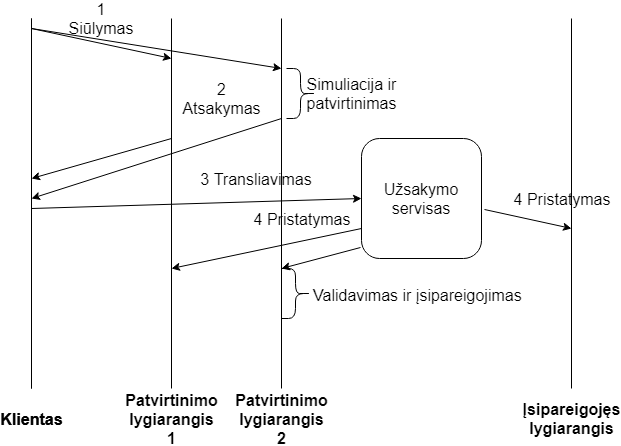
\includegraphics[scale=0.5]{img/MLP}
    \caption{Tranzakcijų sekų diagrama}   % Antraštė įterpiama po paveikslėlio
    \label{img:mlp}
\end{figure}

				
		\subsubsection{Parametrai}

		Mano nurodytuose moksliniuose straipsniuose (\cite{ThailandPerf} \cite{IMBResearch}) darytuose Fabric greičio tyrimuose
		buvo išskirtas parametrų sarašas, kuriuos keičiant mokslininkai išskyrė sąrašą parametrų kuriuos keisdami jie matavo Fabric darbą. 
		Šiame poskiryje autorius trumpai supažindins su šiais parametais ir sekančiame skyriuje pateiks tyrimų duomenis.
			
			\begin{itemize}
				\item{Mazgų skaičius - didėjant mazgų skaičiui tinkle norint patvirtinti bloką trunka ilgiau laiko išsiūti jį visiems tinklo mazgams.}
				\item{Tranzakcijų skaičius - keičiant tranzakcijų skaičiū keičiasi vėlavimas ir pralaidumas}
				\item{Bloko dydis - tranzakcijos yra sugrupuojamos į blokus. Blokai yra siunčiami visiems tinklo perams. Užsakymo parašas 
būna verifikuojamas kiekvienam blokui, o perdavimo patvirtinimo parašas verifikuojamas kiekvienai transakcijai, todėl keičiant bloko dydį atsiranda konmprpisas tarp palaidumo ir vėlavim}
				\item{Patvirtinimo politika - diktuoja kiek tranzakcijų ir pasirašymų turi būti įvykdyta prieš siunčiant tranzakcijas užsakytoją. Didinant politikos sudėtingumą didės resursų sunaudojimas ir įvertinimo laikas.}
				\item{Kanalai - izoliuoja tranzakcijas viena nuo kitos ir norint persiųsti tranzakcijas iš vieno kanalo į kitą turi būti patvirtintos, surikiuotos ir apdorotos nepriklausomai viena nuo kitos.}
				\item{Resursų paskirstymas - kiekvienas peras vykdo grandinės kodą skirtą parašo skaičiavimams ir verifikavimo rutinoms. Keičiant procesoriaus branduolių skaičių keičiasi vykdymo greitis.}
				\item{Būsenos duomenų bazė - Fabric naudoją dvi duomenų bazes, CouchDB ir GoLevelDB, kuriuose galima saugoti ledgerio buseną}
			\end{itemize}

		\subsubsection{Testavimo metodologijos}
			Abiejuose autoriaus apriamose straipsniuose pralaidumas ir vėlavimas yra pagrindinės darbo metrikos. Pirmajame straipsnyje \cite{IMBResearch}  buvo simuliuojamos keturios organizacijos kurios kiekviena iš jų turi po du piersus, iš viso 8 mazgai tinkle. Kiekvienas tinklo klientas pastoviai generuoja tranzakcijas, taip pat pastoviai siųsdamas teikimo užklausas ir patvirtinimo lyginimus. Tranzakcijos yra pateikiamos asinchroniškai. Buvo naudotas jų pačių sukurtas framework'as. Buvo naudoti tokie resursai: x86 64 virtuali mašina IBM SoftLayer duomenų centre. Kiekvienai virtualiai mašinai yra alokuota 32 vCPUs  Intel(R) Xeon(R)
CPU E5-2683 v3 @ 2.00GHz ir 32 GB atminties.  Trys kliento mašinos skirtos generuoti apkrovą buvo alokuota
 56 vCPU ir 128 GB RAM. Mazgai prijungti prie 3 Gbps duomenų centro tinklo. Šiame darbe mokslininkai patys kūrė testavimo frameworką. \\
Antrajame darbe(\cite{ThailandPerf}) buvo naudota: Amazon AWS EC2
 su Intel E5-1650 8 branduolių CPU,
15GB RAM, 128GB SSD. Tyrimui atlikti buvo sukurta pinigų pervedimo aplikacija. Pagrindinis jos funkcionalumas buvo: sukurti paskyrą, išleisti naujus pinigus bei pervesti pinigus iš vienos paskyros į kitą. Kaip ir pirmajame straipsnyje užklausos buvo siunčiamoks asinchroniškai.
 
		\subsubsection{Tyrimų rezultatai}
			\begin{itemize}
				\item{Vėlavimas}
				\item{Pralaidumas}
				\item{Greitis}
			\end{itemize}

	\subsection{MySQL}
	\subsection{PostgreSQL}
\section{Tyrimas}

\section{Žodynas}
\begin{itemize}
	\item{Grandinės kodas(angl. chaincode) - programa parašyta Go, Java arba NodeJS kalbomis kuri vykdo
 verslo logiką sutartą tarp tinklo narių.}
	\item{Peras(angl. peer) - tinklo dalyvis gaunantis ir siunčiantis informaciją.}
\end{itemize}


\printbibliography[heading=bibintoc]  









\end{document}
